\documentclass[9pt,a5paper]{extarticle}
\usepackage[margin=1cm]{geometry}
\usepackage[utf8]{inputenc}
\usepackage[IL2]{fontenc}
\usepackage[czech]{babel}
\usepackage{microtype}
\usepackage{amssymb}
\usepackage{amsthm}
\usepackage{amsmath}
\usepackage{xcolor}
\usepackage{graphicx}

\usepackage[inline]{enumitem}

\newcommand{\R}{\mathbb{R}}

\setlist[enumerate]{label={(\alph*)},topsep=\smallskipamount,itemsep=\smallskipamount,parsep=0pt}
\setlist[itemize]{topsep=\smallskipamount,noitemsep}

\def\tisk{%
\newbox\shipouthackbox
\pdfpagewidth=2\pdfpagewidth
\let\oldshipout=\shipout
\def\shipout{\afterassignment\zdvojtmp \setbox\shipouthackbox=}%
\def\zdvojtmp{\aftergroup\zdvoj}%
\def\zdvoj{%
    \oldshipout\vbox{\hbox{%
        \copy\shipouthackbox
        \hskip\dimexpr .5\pdfpagewidth-\wd\shipouthackbox\relax
        \box\shipouthackbox
    }}%
}}%



\newtheorem*{poz}{Pozorování}

\theoremstyle{definition}
\newtheorem{uloha}{Úloha}
\newtheorem{suloha}[uloha]{\llap{$\star$ }Úloha}
\newtheorem*{bonus}{Bonus}
\newtheorem*{defn}{Definice}

\pagestyle{empty}

\let\=\doteq
\let\ee\expandafter

\def\vysld{}
\let\printvysl\relax

\makeatletter
\long\def\vyslplain#1{\ee\ee\ee\gdef\ee\ee\ee\vysld\ee\ee\ee{\ee\vysld\ee\printvysl\ee{\the\c@uloha}{#1}}}
\let\vysl\vyslplain

\def\locvysl#1{\ee\gdef\ee\locvysld\ee{\locvysld\item #1}}
\let\lv\locvysl

\newenvironment{ulohav}[1][]{\begin{uloha}[#1]\gdef\locvysld{\begin{enumerate*}}}{\ee\vyslplain\ee{\locvysld\end{enumerate*}}\end{uloha}}
\newenvironment{sulohav}[1][]{\begin{suloha}[#1]\gdef\locvysld{\begin{enumerate*}}}{\ee\vyslplain\ee{\locvysld\end{enumerate*}}\end{suloha}}

\makeatother

\begin{document}

%\tisk

\section*{2. Tělesná všehochuť}

\mathcode`\,="013B


\begin{uloha}[Na rozjezd]\label{site}
Rozhodněte, které ze sítí níže jsou sítěmi krychle:
\vyslplain{1, 4, 6, 7, 8, 9, 12, 13, 14 a 15}
\end{uloha}

\begin{uloha}
Pojmenujte tělesa, jejichž sítě jsou níže:
\vyslplain{\begin{enumerate*}
    \item pravidelný čtyřboký jehlan,
    \item kužel,
    \item kvádr,
    \item pravidelný šestiboký jehlan,
    \item pravidelný trojboký hranol,
    \item pravidelný šestiboký hranol,
    \item válec,
    \item pravidelný osmistěn.
\end{enumerate*} (všechny jehlany, kužely, hranoly jsou kolmé)}
\end{uloha}
\vskip-\bigskipamount
\[ \mathbf{1.}\ \vcenter{\hbox{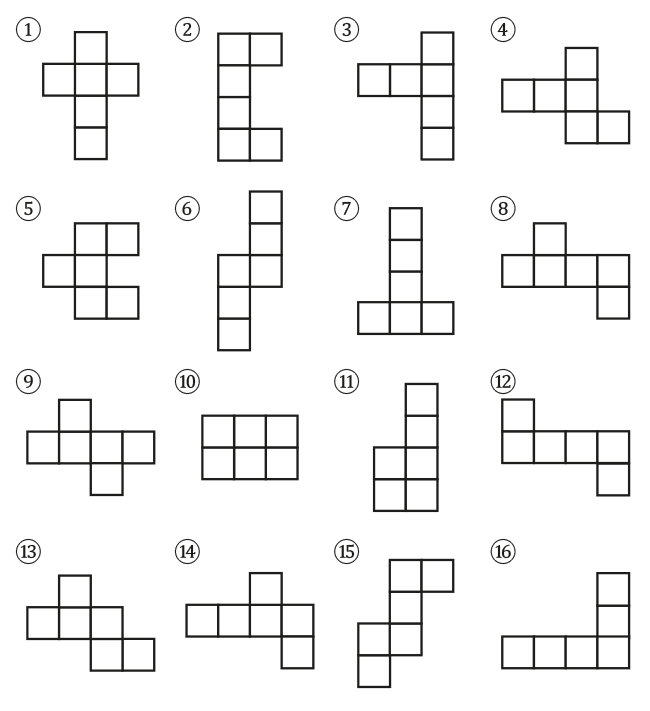
\includegraphics[width=.35\hsize]{cube_nets.png}}} \qquad \mathbf{2.}\  \vcenter{\hbox{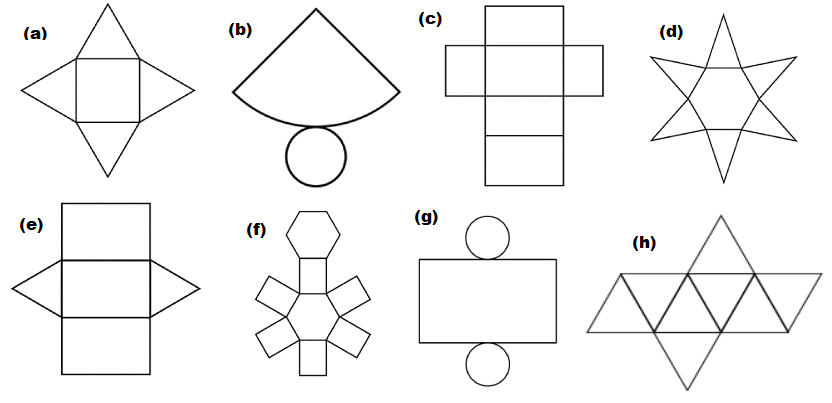
\includegraphics[width=.5\hsize]{site_teles.png}}} \]

\begin{uloha}
Kvádr má rozměry v poměru $1 : 1,5 : 2$ a objem $3000\,\mathrm{cm}^3$. Určete délky jeho stran.
\vyslplain{10, 15, 20}
\end{uloha}

\begin{uloha}
Kvádr má rozměry v poměru $2:3:6$ a tělesovou úhlopříčku délky $14$. Určete jeho objem.
\vyslplain{$288$}
\end{uloha}

\begin{uloha}\label{zvetseni}
Jestliže hranu krychle zvětšíme dvakrát, kolikrát se zvětší její objem? A co povrch?
\vyslplain{objem osmkrát, povrch čtyřikrát}
\end{uloha}

\begin{uloha}
Pro (kolmý) pravidelný šestiboký hranol $ABCDEFA'B'C'D'E'F'$ se stranou $|AB| = 4$ a úhlopříčkou $|AD'| = 10$ určete objem a povrch.
\vyslplain{objem $144\sqrt 3$, povrch $144+48\sqrt3$}
\end{uloha}

\begin{uloha}
Odvoďte vzorec pro objem pravidelného čtyřstěnu, jehož hrana má délku $a$.
\vyslplain{$\dfrac{a^3}{6\sqrt2}$}
\end{uloha}


\begin{uloha}
Určete délku podstavné hrany pravidelného \emph{pětibokého} hranolu, jehož výška je stejná jako délka podstavné hrany a objem je $100$.
\vyslplain{cca 3,874}
\end{uloha}

\begin{uloha}
Nalezněte (platnou) síť krychle, která se nenachází v Úloze \ref{site}.
\vysl{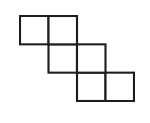
\includegraphics[width=1.5cm]{last_cube_net.png}}
\end{uloha}


\begin{uloha} % 100% realisticky.cz
Na základě Úlohy \ref{zvetseni} zkuste vysvětlit některé z následujících jevů: 
\begin{enumerate}
    \item Vítr zvedá písek (malé kamínky), ale nezvedá větší balvany ze stejného materiálu. 
    \item Mravenec se nezabije ani při pádu ze čtvrtého patra (člověk většinou ano). 
    \item Velikost teplokrevných živočichů většinou vzrůstá se zeměpisnou šířkou jejich výskytu. 
\end{enumerate}
\vyslplain{%
\begin{enumerate}
    \item %Vítr zvedá písek (malé kamínky), ale nezvedá větší balvany ze stejného materiálu. 
Vítr zvedá kamínky odporem vzduchu, který je závislý na ploše kamínku. Zvednutí kamínku 
brání gravitační síla, která odpovídá hmotnosti a tím i objemu kamínku. 
Pokud se kámen zmenší 100 $\times$, jeho plocha se zmenší 10\,000$\times$, ale hmotnost 1000\,000$\times$ $\Rightarrow$ 
s rozměry klesá hmotnost rychleji než plocha a tak u dostatečně malých kamenů převáží 
odpor vzduchu nad gravitací a vítr kamínek zvedne.  
    \item
%Mravenec se nezabije ani při pádu ze čtvrtého patra (člověk většinou ano). 
Podobné jako v předchozím bodu. Pád zrychluje gravitace (závislá na objemu), brzdí ho 
odpor vzduchu (závislý na ploše). Čím je předmět lehčí, tím je poměr plocha/objem větší a 
pád pomalejší. 
    \item
%Velikost teplokrevných živočichů většinou vzrůstá se zeměpisnou šířkou jejich výskytu. 
Teplokrevní živočichové se ve studenějších oblastech musejí vyrovnávat se ztrátou tepla, 
která závisí na jejich povrchu – tedy druhé mocnině rozměru. Velikost vnitřního prostředí, ve 
kterém musí živočich teplotu udržovat, je však rovná objemu těla, tedy třetí mocnině rozměru 
$\Rightarrow$ pro živočichy je výhodnější větší rozměr, protože větší tělo má vzhledem k objemu menší 
povrch a tedy i tepelné ztráty.
\end{enumerate}
}
\end{uloha}

\begin{uloha}
Odvoďte vzorec $V = \frac13 v (S_1 + S_2 + \sqrt{S_1 S_2})$ pro objem komolého jehlanu, jehož podstavy mají obsahy $S_1$ a $S_2$. Návod: Objem chceme vyjádřit jako rozdíl objemů dvou jehlanů s podstavami o obsazích $S_1$ a $S_2$ a výškách $v_1$ a $v_2$; jednak určitě platí $v = v_1 - v_2$, dále $S_1 : S_2 = v_1^2 : v_2^2$, což se dá výhodně přepsat jako $\sqrt{S_1} : \sqrt{S_2} = v_1 : v_2$.
\end{uloha}


\newpage
\parindent=0pt
\parskip=\smallskipamount
\def\printvysl#1#2{\textbf{#1.}\ #2\par}
\vysld



\end{document}